% Smart Sign Language Gloves (SSLG) - Final Project Report
\documentclass[12pt,a4paper]{report}

% ── Packages ────────────────────────────────────────────────────────────────
\usepackage[a4paper,left=1.5in,right=1in,top=1in,bottom=1in]{geometry}
\usepackage{setspace}
\usepackage{graphicx}
\usepackage{float}
\usepackage{caption}
\usepackage{subcaption}
\usepackage{booktabs}
\usepackage{tabularx}
\usepackage{array}
\usepackage{longtable}
\usepackage{amsmath}
\usepackage{enumitem}
\usepackage{url}
\usepackage[hidelinks]{hyperref}
\usepackage{newtxtext}
\usepackage{newtxmath}
\usepackage{ragged2e}
\usepackage{fancyhdr}
\usepackage{titlesec}
\usepackage{tikz}
\usetikzlibrary{arrows.meta,positioning,shapes.geometric,shapes.misc,calc,fit,backgrounds,shadows}

\onehalfspacing
\setlength{\parskip}{0.5em}
\setlength{\parindent}{0pt}
\justifying

% ── Header / Footer ─────────────────────────────────────────────────────────
\pagestyle{fancy}
\fancyhf{}
\cfoot{\thepage}
\renewcommand{\headrulewidth}{0pt}
\renewcommand{\footrulewidth}{0pt}

% ── Heading styles ──────────────────────────────────────────────────────────
\titleformat{\chapter}[display]
  {\bfseries\Large}
  {\chaptername\ \thechapter}
  {0.5em}
  {}
\titleformat{\section}{\bfseries\large}{\thesection}{0.75em}{}
\titleformat{\subsection}{\bfseries\normalsize}{\thesubsection}{0.75em}{}

% ── Colour palette (from research paper) ─────────────────────────────────────
\definecolor{colTeal50}   {HTML}{E1F5EE}
\definecolor{colTeal600}  {HTML}{0F6E56}
\definecolor{colTeal800}  {HTML}{085041}
\definecolor{colBlue50}   {HTML}{E6F1FB}
\definecolor{colBlue600}  {HTML}{185FA5}
\definecolor{colBlue800}  {HTML}{0C447C}
\definecolor{colAmber50}  {HTML}{FAEEDA}
\definecolor{colAmber600} {HTML}{854F0B}
\definecolor{colAmber800} {HTML}{633806}
\definecolor{colPurple50} {HTML}{EEEDFE}
\definecolor{colPurple600}{HTML}{534AB7}
\definecolor{colPurple800}{HTML}{3C3489}
\definecolor{colGray50}   {HTML}{F1EFE8}
\definecolor{colGray600}  {HTML}{5F5E5A}
\definecolor{colGray800}  {HTML}{444441}
\definecolor{colGreen50}  {HTML}{EAF3DE}
\definecolor{colGreen600} {HTML}{3B6D11}
\definecolor{colGreen800} {HTML}{27500A}
\definecolor{colCoral50}  {HTML}{FAECE7}
\definecolor{colCoral600} {HTML}{993C1D}
\definecolor{colCoral800} {HTML}{712B13}

% ── TikZ block-diagram styles ────────────────────────────────────────────────
\tikzset{
  block/.style={
    draw, rounded corners=5pt,
    minimum width=36mm, minimum height=13mm,
    align=center, inner sep=5pt,
    line width=0.5pt, font=\scriptsize\sffamily
  },
  sensor/.style  ={block, fill=colBlue50,    draw=colBlue600},
  mcu/.style     ={block, fill=colTeal50,    draw=colTeal600},
  power/.style   ={block, fill=colAmber50,   draw=colAmber600},
  wifi/.style    ={block, fill=colPurple50,  draw=colPurple600},
  backend/.style ={block, fill=colGray50,    draw=colGray600},
  webui/.style   ={block, fill=colGreen50,   draw=colGreen600},
  ml/.style      ={block, fill=colCoral50,   draw=colCoral600},
  mainarr/.style ={
    -{Stealth[length=2.2mm,width=1.4mm]},
    line width=0.9pt, draw=colGray600
  }
}

\newcommand{\nodetext}[4]{%
  {\color{#1}\textbf{#2}}\\[1.5pt]%
  {\color{#3}\scriptsize #4}%
}

% ── Project metadata ─────────────────────────────────────────────────────────
\newcommand{\SystemName}{Smart Sign Language Gloves: A Real-Time ISL-to-Speech Translation System}
\newcommand{\SystemAcronym}{SSLG}
\newcommand{\InstituteName}{Vidyavardhini's College Of Engineering \& Technology, Vasai Road}
\newcommand{\DeptName}{Department of Electronics and Telecommunication Engineering}
\newcommand{\UniversityName}{University of Mumbai}
\newcommand{\TeamMemberA}{Kushagra Naresh Joshi}
\newcommand{\TeamMemberB}{Afroz Abdul Inamdar}
\newcommand{\TeamMemberC}{Sakshi Rajendra Jagdale}
\newcommand{\TeamMemberD}{Ramzan Badruduja Khan}
\newcommand{\GuideName}{Ms.\ Shaista Khan}
\newcommand{\ProjectType}{Semester Project Report}
\newcommand{\SubmissionDate}{March 2026}
\newcommand{\AcademicYear}{2025--2026}

\begin{document}

% ── Title Page ───────────────────────────────────────────────────────────────
\begin{titlepage}
  \thispagestyle{empty}
  \centering
  \vspace*{0.6in}
  \IfFileExists{vect.png}{
\includegraphics[width=0.22\textwidth]{vect.png}\\[0.2in]}{}
  {\Large\textbf{\InstituteName}}\\[0.1in]
  {\large\textbf{\DeptName}}\\[0.15in]
  {\large\textbf{\UniversityName}}\\[0.35in]

  {\Large\textbf{\ProjectType}}\\[0.15in]
  {\Large\textbf{\SystemName}}\\[0.35in]

  {\large\textbf{Submitted in partial fulfillment of the requirements}}\\
  {\large\textbf{for the degree of Bachelor of Engineering}}\\[0.2in]
  {\large\textbf{(Electronics and Telecommunication Engineering)}}\\[0.35in]

  {\large\textbf{Submitted by}}\\[0.1in]
  {\large \TeamMemberA}\\
  {\large \TeamMemberB}\\
  {\large \TeamMemberC}\\
  {\large \TeamMemberD}\\[0.3in]

  {\large\textbf{Project Guide}}\\
  {\large \GuideName}\\[0.3in]

  {\large\textbf{Academic Year:} \AcademicYear}\\[0.15in]
  {\large\textbf{\SubmissionDate}}\\
\end{titlepage}

\cleardoublepage
\pagenumbering{roman}
\setcounter{page}{1}

% ── Certificate Page ─────────────────────────────────────────────────────────
\chapter*{Certificate}
\addcontentsline{toc}{chapter}{Certificate}
This is to certify that the project report entitled \textbf{\SystemName} is a bona fide
work carried out by \textbf{\TeamMemberA}, \textbf{\TeamMemberB},
\textbf{\TeamMemberC}, and \textbf{\TeamMemberD} of the
\DeptName, \InstituteName, \UniversityName, for the partial
fulfillment of the requirements for the degree of Bachelor of Engineering
in Electronics and Telecommunication Engineering during the academic year
\AcademicYear. The work is satisfactory and has not been submitted
previously for any degree or diploma.

\vspace{1in}
\textbf{Subject Incharge / Project Guide}\\
\GuideName\\
(Signature)

\cleardoublepage

% ── Declaration Page ────────────────────────────────────────────────────────
\chapter*{Declaration}
\addcontentsline{toc}{chapter}{Declaration}
We, \textbf{\TeamMemberA}, \textbf{\TeamMemberB}, \textbf{\TeamMemberC}, and
\textbf{\TeamMemberD}, hereby declare that the project report entitled
\textbf{\SystemName} submitted to \UniversityName is a record of original work
carried out by us under the guidance of \GuideName. The work reported
herein has not been submitted to any other University or Institute for
any degree or diploma.

\vspace{1in}
\begin{tabularx}{\textwidth}{X X}
\textbf{\TeamMemberA} & \textbf{\TeamMemberB} \\
(Signature) & (Signature) \\
\end{tabularx}

\vspace{0.5in}
\begin{tabularx}{\textwidth}{X X}
\textbf{\TeamMemberC} & \textbf{\TeamMemberD} \\
(Signature) & (Signature) \\
\end{tabularx}

\cleardoublepage

% ── Abstract ────────────────────────────────────────────────────────────────
\chapter*{Abstract}
\addcontentsline{toc}{chapter}{Abstract}
Indian Sign Language (ISL) remains inaccessible to most non-signers, creating
persistent communication barriers. \SystemName (\SystemAcronym) is a wearable
ISL-to-speech translation system that produces real-time text and spoken output
from hand gestures. The glove employs Hall-effect sensing with fingertip magnets
and a 6-axis inertial measurement unit (IMU), sampled by an ATmega328P
microcontroller. Sensor frames are transmitted over Wi-Fi using an ESP8266 to a
Flask backend that manages data collection, model training, and inference. A
CNN--LSTM model classifies 20 ISL gestures. Experimental evaluation in controlled
laboratory conditions yielded 82--90\% classification accuracy with an end-to-end
latency of 220--320 ms. The system demonstrates a low-cost, portable approach to
ISL translation with a scalable improvement path through continuous data
collection and model updates.

\cleardoublepage

% ── Acknowledgement ─────────────────────────────────────────────────────────
\chapter*{Acknowledgement}
\addcontentsline{toc}{chapter}{Acknowledgement}
We express our sincere gratitude to \textbf{\GuideName} for her valuable
guidance and encouragement throughout this project. We are also thankful to the
\textbf{\DeptName}, \textbf{\InstituteName}, for providing the necessary
facilities and resources. Finally, we thank our friends and families for their
support and motivation.

\cleardoublepage

% ── TOC, Lists ──────────────────────────────────────────────────────────────
\tableofcontents
\listoffigures
\addcontentsline{toc}{chapter}{List of Figures}
\listoftables
\addcontentsline{toc}{chapter}{List of Tables}
\cleardoublepage

% ── Abbreviations ────────────────────────────────────────────────────────────
\chapter*{List of Abbreviations}
\addcontentsline{toc}{chapter}{List of Abbreviations}
\begin{tabularx}{\textwidth}{@{}lX@{}}
\toprule
\textbf{Abbreviation} & \textbf{Description} \\
\midrule
ISL & Indian Sign Language \\
SSLG & Smart Sign Language Gloves \\
IMU & Inertial Measurement Unit \\
MCU & Microcontroller Unit \\
ADC & Analog-to-Digital Converter \\
CNN & Convolutional Neural Network \\
LSTM & Long Short-Term Memory \\
UART & Universal Asynchronous Receiver/Transmitter \\
\bottomrule
\end{tabularx}
\cleardoublepage
\pagenumbering{arabic}
\setcounter{page}{1}

% ── Chapter 1: Introduction ─────────────────────────────────────────────────
\chapter{Introduction}
\section{Background}
Sign language is the primary mode of communication for many hearing-impaired
individuals. However, most non-signers are unable to understand ISL, which
creates a communication gap in everyday interactions. The goal of this project
is to bridge that gap using a wearable, low-cost translation system.

\section{Problem Statement}
Camera-based solutions can achieve good recognition rates but are sensitive to
lighting, occlusion, and framing. Flex-sensor gloves offer portability but can
suffer from mechanical drift and degradation. A robust and repeatable glove
using Hall-effect sensors, combined with a scalable backend for model updates,
can improve reliability and maintainability for ISL translation.

\section{Objectives}
\begin{itemize}[noitemsep]
  \item Design a wearable glove using Hall-effect sensors and IMU data.
  \item Capture and transmit multi-channel gesture data over Wi-Fi.
  \item Train a CNN--LSTM model for 20 ISL gestures.
  \item Provide real-time text and speech output through a web interface.
  \item Validate accuracy, latency, and battery autonomy.
\end{itemize}

\section{Scope}
This work focuses on 20 commonly used ISL gestures, laboratory evaluation, and
adult volunteers with consistent sensor placement. The design is intended for
future expansion to a larger vocabulary and more diverse users.

\section{Organization of the Report}
Chapter 2 covers related work, Chapter 3 presents requirements, Chapter 4
explains system design, Chapter 5 describes methodology, Chapter 6 details
implementation, Chapter 7 provides results and discussion, and Chapter 8
concludes with future scope.

% ── Chapter 2: Literature Review ─────────────────────────────────────────────
\chapter{Literature Review}
\section{Vision-Based Approaches}
Camera-based gesture recognition systems provide rich visual features but require
controlled lighting and clear framing. They are sensitive to occlusion and can
be computationally expensive for real-time deployment.

\section{Sensor-Based Gloves}
Glove-based systems directly capture finger and hand movement. Earlier flex
sensor designs are simple but can degrade with repeated bending and show
non-linear drift. Hall-effect sensing offers non-contact measurement with better
durability and stability.

\section{Identified Gaps}
Many prior systems do not address calibration time, sensor drift, or the
workflow required to label data and update models. \SystemAcronym addresses these
gaps through a repeatable calibration routine, structured dataset management,
and a retrainable backend pipeline.

% ── Chapter 3: Requirements ─────────────────────────────────────────────────-
\chapter{System Requirements}
\section{Hardware Requirements}
\begin{itemize}[noitemsep]
  \item ATmega328P microcontroller
  \item Hall-effect sensors (SS49E) with fingertip magnets
  \item MPU-6050 IMU (6-axis)
  \item ESP8266 Wi-Fi module (ESP-01)
  \item 18650 Li-ion battery with TP4056 charger
  \item MT3608 boost converter and LM2596 buck converter
\end{itemize}

\section{Software Requirements}
\begin{itemize}[noitemsep]
  \item Embedded firmware for data acquisition and UART framing
  \item Python Flask backend for ingestion, labeling, training, and inference
  \item Model training using TensorFlow / Keras
  \item Web interface for live display and dataset management
\end{itemize}

% ── Chapter 4: System Design ────────────────────────────────────────────────
\chapter{System Design}
\section{Overall Architecture}
The system is composed of a glove-side sensing layer and a backend inference
layer. The glove acquires Hall sensor and IMU signals, frames them on the MCU,
and transmits data over Wi-Fi. The backend performs preprocessing, model
training, and inference and returns text/speech outputs.

\begin{figure}[H]
  \centering
  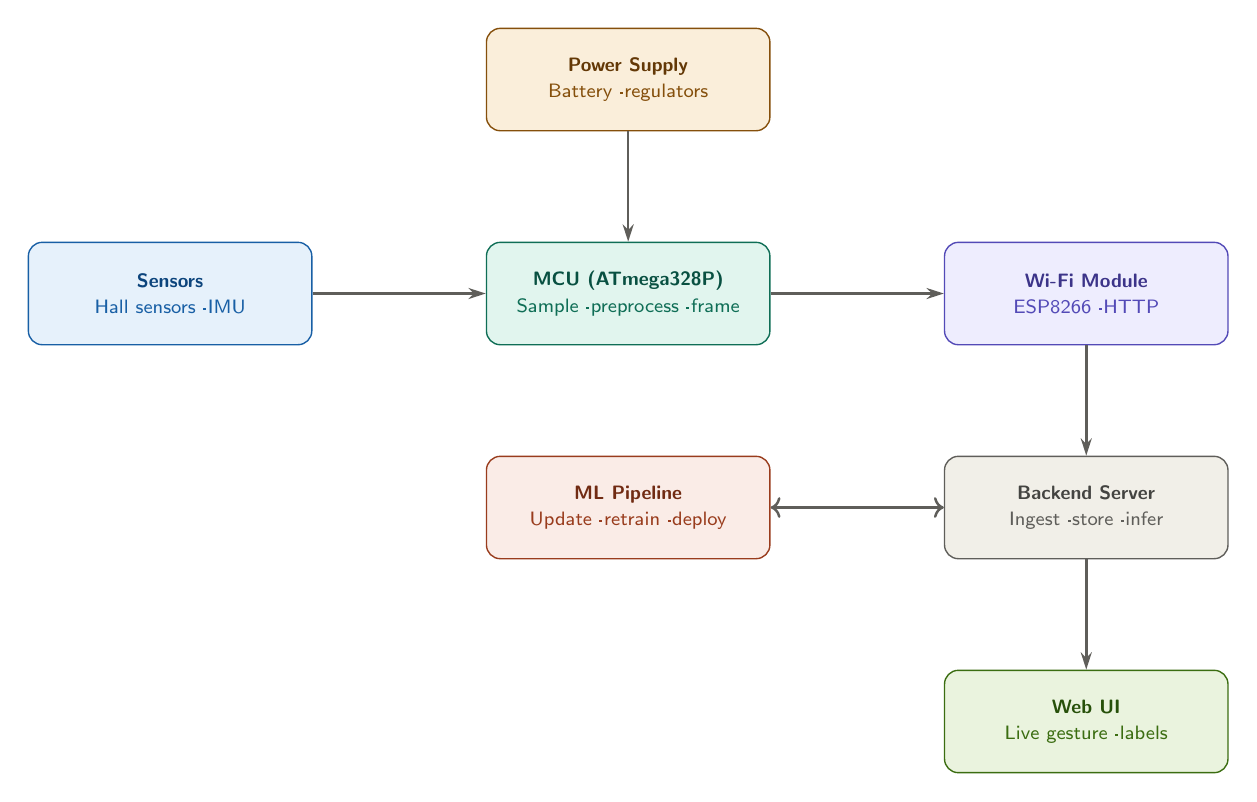
\begin{tikzpicture}[
      node distance = 14mm and 22mm,
      every node/.style={font=\scriptsize\sffamily}
  ]
    \node[sensor] (sens) {\nodetext{colBlue800}{Sensors}{colBlue600}{Hall sensors \textperiodcentered IMU}};
    \node[mcu, right=22mm of sens] (mcu) {\nodetext{colTeal800}{MCU (ATmega328P)}{colTeal600}{Sample \textperiodcentered preprocess \textperiodcentered frame}};
    \node[wifi, right=22mm of mcu] (wifi) {\nodetext{colPurple800}{Wi-Fi Module}{colPurple600}{ESP8266 \textperiodcentered HTTP}};
    \node[power, above=14mm of mcu] (pwr) {\nodetext{colAmber800}{Power Supply}{colAmber600}{Battery \textperiodcentered regulators}};
    \node[backend, below=14mm of wifi] (backend) {\nodetext{colGray800}{Backend Server}{colGray600}{Ingest \textperiodcentered store \textperiodcentered infer}};
    \node[webui, below=14mm of backend] (webui) {\nodetext{colGreen800}{Web UI}{colGreen600}{Live gesture \textperiodcentered labels}};
    \node[ml, below=14mm of mcu] (ml) {\nodetext{colCoral800}{ML Pipeline}{colCoral600}{Update \textperiodcentered retrain \textperiodcentered deploy}};

    \draw[mainarr] (sens.east) -- (mcu.west);
    \draw[mainarr] (pwr.south) -- (mcu.north);
    \draw[mainarr] (mcu.east) -- (wifi.west);
    \draw[mainarr] (wifi.south) -- (backend.north);
    \draw[mainarr] (backend.south) -- (webui.north);
    \draw[mainarr,<->] (backend.west) -- (ml.east);
  \end{tikzpicture}
  \caption{End-to-end system architecture of \SystemAcronym.}
\end{figure}

\section{Communication Protocol}
Sensor frames are transmitted from the MCU to the ESP8266 over UART at 115200 bps.
The ESP8266 forwards the frames to the backend via HTTP POST. A lightweight
acknowledgment using HTTP status codes detects packet loss and supports retries.

\begin{table}[H]
  \centering
  \caption{UART packet format (MCU to Wi-Fi module)}
  \begin{tabularx}{\textwidth}{@{}lcX@{}}
    \toprule
    Field & Bytes & Description \\
    \midrule
    Preamble       & 1  & 0xAA sync byte \\
    Version        & 1  & Protocol version \\
    Timestamp      & 2  & Milliseconds mod 65536 \\
    Gesture[0--4]  & 10 & 5 channels, 2 bytes each (ADC) \\
    IMU[0--5]      & 12 & 6 axes, 2 bytes each \\
    Label ID       & 1  & Optional during collection mode \\
    Checksum       & 1  & XOR of all payload bytes \\
    \midrule
    \textbf{Total} & \textbf{28} & \\
    \bottomrule
  \end{tabularx}
\end{table}

\section{Circuit Overview}
\begin{figure}[H]
  \centering
  \IfFileExists{KICAD_SL_PDF.pdf}{%
    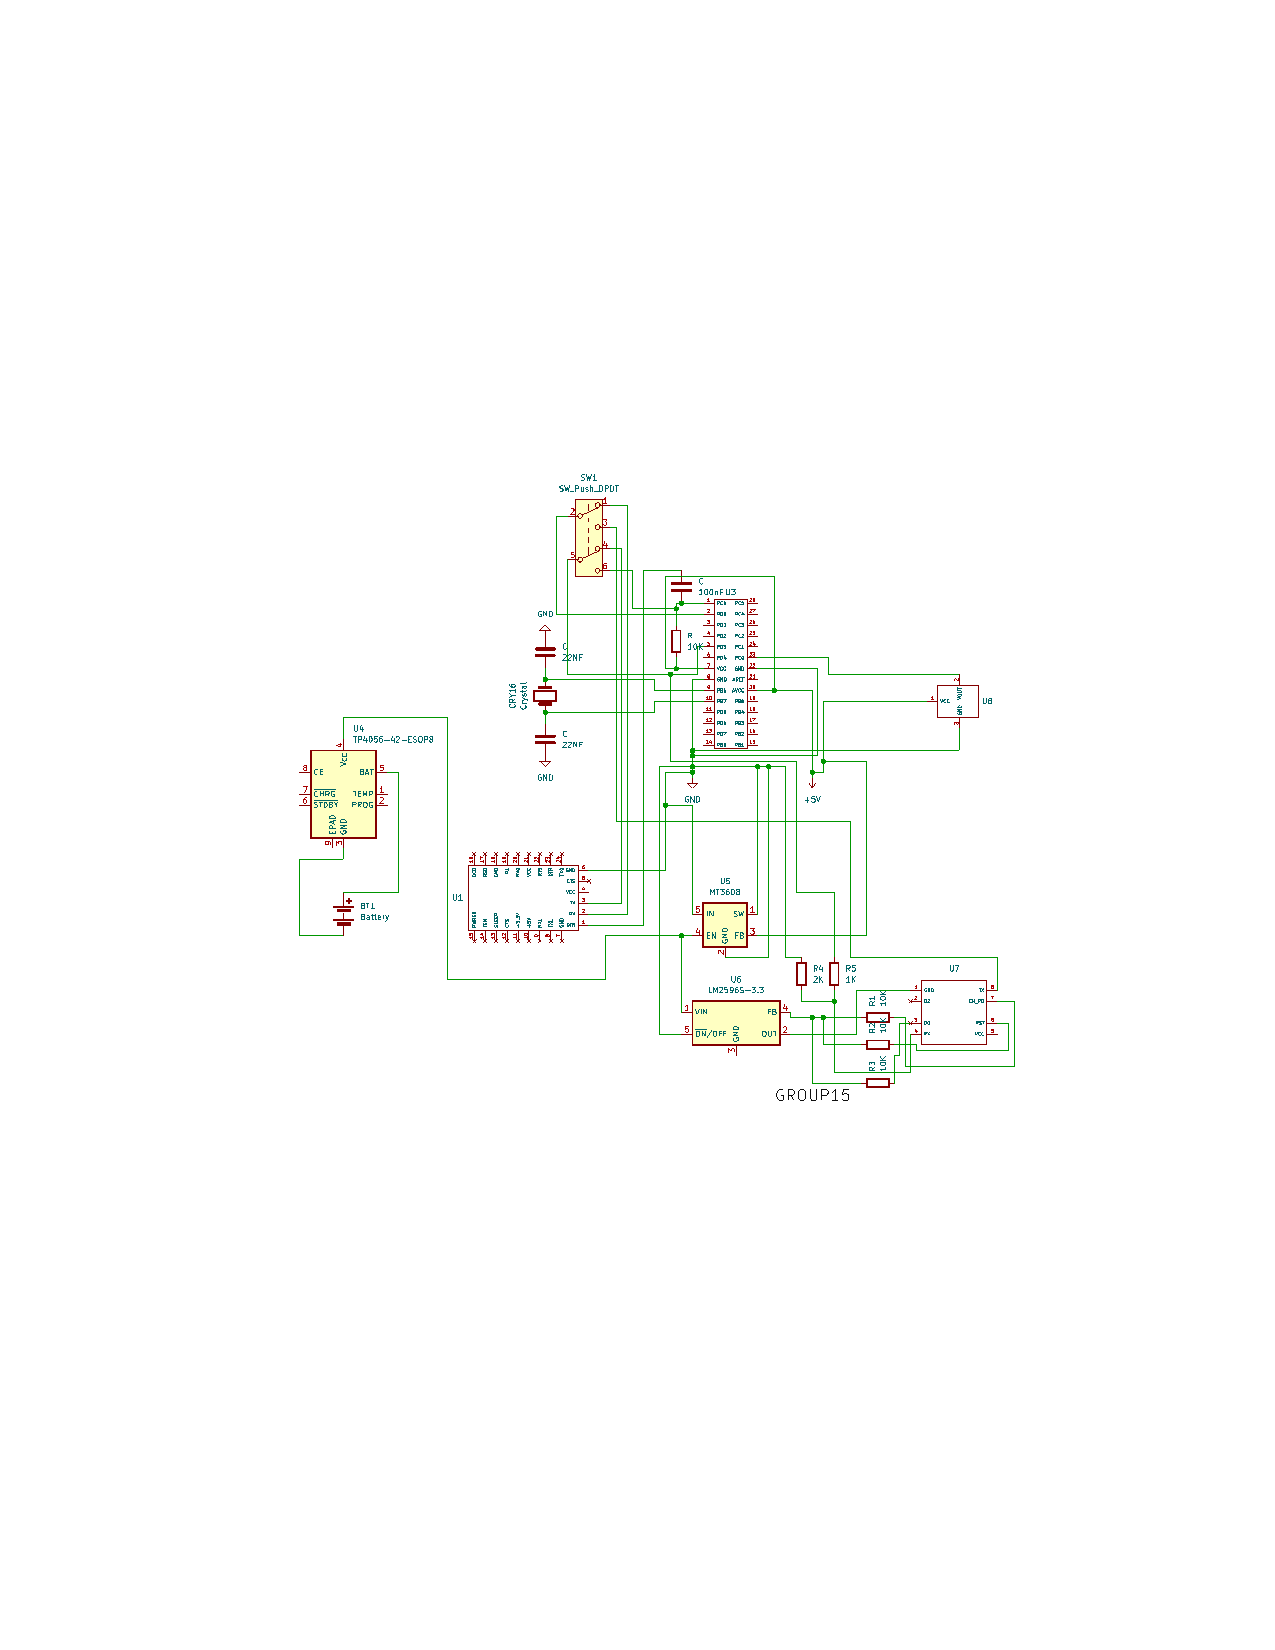
\includegraphics[page=1,width=0.95\textwidth,height=0.70\textheight,keepaspectratio,trim=40mm 85mm 40mm 80mm,clip]{KICAD_SL_PDF.pdf}%
  }{%
    \fbox{\parbox{0.9\textwidth}{\centering Circuit diagram placeholder}}
  }%
  \caption{Complete circuit schematic of \SystemAcronym.}
\end{figure}

% ── Chapter 5: Methodology ─────────────────────────────────────────────────-
\chapter{Methodology}
\section{Calibration}
Before each session, the user holds a neutral open-palm pose for 3 seconds. The
firmware computes a per-channel baseline $b_i$ and stores it in EEPROM. All
subsequent readings use $\Delta_i = x_i - b_i$, ensuring the classifier learns
pose-relative patterns rather than absolute ADC levels.

\section{Windowing and Feature Formation}
The sensor stream is segmented into overlapping windows of $W$ samples (25--50)
with 50\% overlap. Each window produces a tensor of shape $W \times C$, where
$C=11$ channels (5 Hall sensors + 6 IMU axes). This representation captures
temporal variations in ISL gestures.

\section{Model Architecture}
A CNN--LSTM architecture is used:
\begin{itemize}[noitemsep]
  \item Two 1-D convolutional layers (kernel size 3; 32 and 64 filters) with ReLU.
  \item One LSTM layer with 128 units.
  \item Dense softmax output for 20 gesture classes.
\end{itemize}
Dropout (0.4) mitigates overfitting. The trained model is quantized for fast
inference.

% ── Chapter 6: Implementation ───────────────────────────────────────────────-
\chapter{Implementation}
\section{Firmware}
The ATmega328P samples five Hall sensors and the IMU, applies baseline
subtraction and light filtering, and transmits framed packets over UART. The
ESP8266 module handles Wi-Fi and HTTP communication with the backend.

\section{Backend}
A Flask server manages data ingestion, labeling, preprocessing, training, and
inference. The web interface provides live gesture display and a labeling
workflow for iterative dataset growth.

\section{Dataset}
Volunteers perform each gesture across multiple sessions. The dataset is stored
as CSV with sensor values, labels, and session metadata. Oversampling balances
under-represented classes to target approximately 1000 samples per gesture.

\begin{table}[H]
  \centering
  \caption{CSV column schema}
  \begin{tabularx}{\textwidth}{@{}lX@{}}
    \toprule
    Column & Description \\
    \midrule
    ts\_ms          & Timestamp (milliseconds) \\
    gesture0..4     & Raw Hall-effect ADC channels (5) \\
    ax, ay, az      & Accelerometer axes \\
    gx, gy, gz      & Gyroscope axes \\
    label\_id       & Gesture identifier (integer) \\
    label\_name     & Gesture name (string) \\
    participant\_id & Anonymous participant ID \\
    session\_id     & Session identifier \\
    \bottomrule
  \end{tabularx}
\end{table}

% ── Chapter 7: Testing and Results ─────────────────────────────────────────-
\chapter{Testing and Results}
\section{Experimental Setup}
Experiments were conducted in a university laboratory using a dedicated 2.4 GHz
access point. The backend ran on an Intel Core i5-class laptop with 8 GB RAM.
Each session began with the 3-second open-palm calibration. End-to-end latency
was measured from sensor packet capture to inference response.

\section{Performance Metrics}
\begin{table}[H]
  \centering
  \caption{Measured performance metrics}
  \begin{tabularx}{\textwidth}{@{}lX@{}}
    \toprule
    Metric & Value \\
    \midrule
    Accuracy (\%)                 & 82 -- 90 \\
    Precision                     & 0.87 \\
    Recall                        & 0.91 \\
    F1-score                      & 0.91 -- 0.93 \\
    Avg. end-to-end latency (ms)  & 220 -- 320 \\
    Peak end-to-end latency (ms)  & 450 -- 650 \\
    Battery autonomy (hours)      & 3 -- 5 \\
    \bottomrule
  \end{tabularx}
\end{table}

\section{Discussion}
Hall-effect sensing reduces mechanical wear compared to flex-based approaches
and provides stable readings when magnet placement is consistent. The web-based
labelling workflow simplifies iterative data collection and model updates. Key
practical challenges include repeatable magnet placement, robust calibration in
real-world environments, and occasional Wi-Fi packet loss.

% ── Chapter 8: Conclusion and Future Scope ─────────────────────────────────-
\chapter{Conclusion and Future Scope}
\section{Conclusion}
\SystemAcronym demonstrates the feasibility of a portable, low-cost ISL
translation system. A Hall-effect sensor glove with an integrated IMU feeds an
ATmega328P sampling layer, which transmits frames over Wi-Fi to a backend
CNN--LSTM inference engine that returns text and speech output. Experimental
results confirm 82--90\% classification accuracy with 220--320 ms end-to-end
latency under laboratory conditions.

\section{Future Scope}
\begin{itemize}[noitemsep]
  \item Expand the gesture vocabulary and user population for broader coverage.
  \item Integrate on-device inference (e.g., TensorFlow Lite) to reduce network dependency.
  \item Improve automatic recalibration and long-term drift compensation.
\end{itemize}

% ── References ──────────────────────────────────────────────────────────────
\begin{thebibliography}{99}
\bibitem{mitra} S. Mitra and T. Acharya, ``Gesture recognition: A survey,'' \textit{IEEE Trans. Syst., Man, Cybern. Part C}, vol. 37, no. 3, pp. 311--324, May 2007. [Online]. Available: \url{https://ieeexplore.ieee.org/document/4154947}
\bibitem{tensorflow} TensorFlow Lite, ``TensorFlow Lite guide,'' 2024. [Online]. Available: \url{https://www.tensorflow.org/guide}
\bibitem{atmega328p} Microchip Technology, ``8-bit microcontroller datasheet,'' 2016. [Online]. Available: \url{https://www.microchip.com/en-us/product/ATmega328P}
\bibitem{ft232rl} FTDI, ``USB-to-UART converter IC.'' [Online]. Available: \url{https://ftdichip.com/products/ft232rl/}
\bibitem{tp4056} ``Single-cell Li-ion battery charger IC datasheet.'' [Online]. Available: \url{https://img.eecart.com/dev/file/part/spec/TP4056-XUNDE.pdf}
\bibitem{battery18650} ``Lithium-ion cylindrical cell overview.'' [Online]. Available: \url{https://en.wikipedia.org/wiki/18650_battery}
\bibitem{mt3608} ``Boost converter IC datasheet.'' [Online]. Available: \url{https://www.ic-components.com/blog/mt3608-step-up-converter-datasheet,pinout,and-applications.jsp}
\bibitem{lm2596} Texas Instruments, ``Buck (step-down) power converter datasheet.'' [Online]. Available: \url{https://www.ti.com/lit/ds/symlink/lm2596.pdf}
\bibitem{esp8266} Espressif Systems, ``Wi-Fi module datasheet,'' 2019. [Online]. Available: \url{https://www.espressif.com/sites/default/files/documentation/0a-esp8266ex_datasheet_en.pdf}
\bibitem{ss49e} Honeywell, ``Linear Hall-effect sensor datasheet.'' [Online]. Available: \url{https://www.mouser.com/datasheet/2/187/SS49E-1122400.pdf}
\bibitem{mpu6050} TDK InvenSense, ``6-axis IMU product specification,'' 2015. [Online]. Available: \url{https://robu.in/wp-content/uploads/2014/12/GY-87_EN.pdf}
\bibitem{flask} Pallets Projects, ``Flask documentation,'' 2024. [Online]. Available: \url{https://flask.palletsprojects.com/en/2.2.x/}
\end{thebibliography}

\end{document}
